\documentclass{article}
\usepackage{titling}
\usepackage[utf8]{inputenc}
\usepackage{hyperref}
\usepackage[letterpaper, portrait, margin=1in]{geometry}
\usepackage{enumitem}
\usepackage{threeparttable}
\usepackage{amsmath}
\usepackage{booktabs}
\usepackage{graphicx}
\usepackage{authblk}

\usepackage{hyperref}
\hypersetup{
colorlinks=true,
    linkcolor=black,
    filecolor=black,      
    urlcolor=blue,
    citecolor=black,
}
\usepackage{natbib}

\usepackage{titlesec}

\title{Homework 4 Solutions}
\author{Kelly Lifchez}
\date{February 10, 2025}
  
\begin{document}
  
\maketitle


\section{Python}

\subsection{Trend Plot} 

\begin{figure}[!ht]
    \centering
    \caption{Treatment Level Trends between January 2017 and December 2018}
    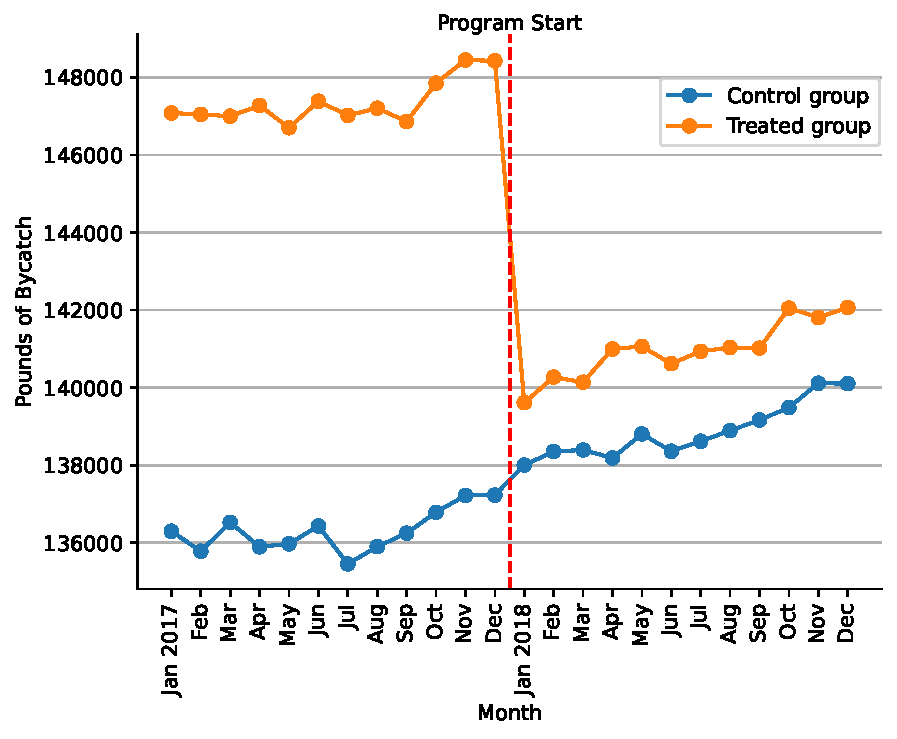
\includegraphics[scale = 0.75]{trend_plot.pdf}
    \begin{minipage}{0.72\textwidth}
        \footnotesize Note: The figure depicts the average pounds of bycatch caught by treated and untreated firms Between January 2017 and December 2018. The green dashed line indicates the start of the bycatch reduction program in January 2018. 
    \end{minipage}
    \label{fig:ame_plot}
\end{figure}

The treated group and control group appear to have parallel trends in average bycatch during the pre-program period (January 2017 to December 2017). 

\newpage
\subsection{Difference in Differences Estimate and Estimator}

Estimating the treatment effect using DID in "manual mode" allows us to see the intuition behind the estimation. The DID estimator compares changes in the bycatch outcome over time between the treated and control groups. Essentially, it takes the observed difference between the treated and control group in the post-program period and the difference between the treated and control group in the pre-program period. Then it finds the difference between these two values, and this difference is the estimated impact of the program. This design works because the trends for both treated and control groups are parallel in the pre-period, meaning we can assume the treated group would have continued along the same trends in the absence of treatment and, therefore, offers a credible counterfactual comparison. This means that we can interpret the DID estimate as the amount by which the program reduced bycatch. in other words, the program led to a reduction in bycatch of approximately -9,591 pounds for treated firms. 

\begin{table}[ht]
\centering
\caption{Treatment Effect of Program on Bycatch}
\vspace{0.3cm}
\begin{threeparttable}
\begin{tabular}{l}
\toprule
DID Estimate \\
\midrule
-9591.35 \\
\bottomrule
\end{tabular}

\end{threeparttable}  
\label{tab:did_est}
\end{table}

\subsubsection*{a) Estimate the treatment effect of the program on bycatch using a regression-based two-period difference-in-differences estimator with estimating equation: $bycatch_{i,t} = \alpha + \lambda_{t=2017} + \gamma g(i) + \delta treat_{i,t} + \epsilon_{i,t}$}

See column 1 of Table \ref{tab:py_regs}.

\subsubsection*{b) Using the full monthly sample, estimate the treatment effect of the program on bycatch using a regression-based DID estimator using the regression: $bycatch_{i,t} = \alpha + \lambda_t + \gamma g(i) + \delta treat_{i,t} + \epsilon_{i,t}$ where $\lambda_t$ are indicator variables for each time period. Report and interpret the results using the same cluster-robust standard errors. How did your results change?}

The magnitude (absolute value) of the coefficient on the treatment indicator decreased slightly, meaning that some of the variation that we thought was caused by the treatment effect based on column (1) was actually caused by month-specific factors or events. 

\subsubsection*{c) Now you want to control for firm size and other covariates that change over time. Estimate the DID regression with added controls: $bycatch_{i,t} = \alpha + \lambda_t + \gamma g(i) + \delta treat_{i,t} + \beta X_{i,t} + \epsilon_{i,t}$
where $X_{i,t}$ includes firm size, pounds of shrimp harvested by firm $i$ in month $t$, and pounds of salmon harvested by firm $i$ in month $t$. Report and interpret the results using the same cluster- robust standard errors. How do your results change from question 1?}

The magnitude of the coefficient decreases again in terms of absolute value, indicating that some of the variation in the model was caused by factors besides the treatment, such as firm size and type of fish. Adding firm-specific indicators appears to have made the estimate more precise, as the standard error on the treatment coefficient in column (3) has decreased by a relatively significant amount as well. The volume of shrimp and salmon are statistically significant and have positive signs, which is unsurprising - I would expect that catching more fish would lead to catching more bycatch. The coefficient on the shrimp variable is larger than the coefficient on the salmon variable, which also makes sense because shrimp boats use trawlers that pick up everything in their paths. 

\subsubsection*{d) Report the results from (a), (b), and (c). How do these results compare to your previous calculations?}

The results shown in column (a) match the estimates produced using "manual" DID calculations. When we add month and firm fixed effects, and especially when we add covariates to control for potential confounders, we get different results. The coefficient on the treatment indicator is still statistically significant, negative, and large in magnitude. Columns (b) and (c) simply offer more precision by parceling out variation caused by factors other than the treatment. 

\vspace{-0.2cm}

\begin{table}[ht]
\centering
\caption{Treatment Effect of Program on Bycatch}
\vspace{0.3cm}
\begin{threeparttable}
\begin{table}
\caption{}
\label{}
\begin{center}
\begin{tabular}{llll}
\hline
               & (a)           & (b)           & (c)           \\
\hline
Intercept      & 138001.814*** & 136154.047*** & 1547.006      \\
               & (18657.796)   & (18371.139)   & (1105.822)    \\
pre            & -773.216      &               &               \\
               & (598.685)     &               &               \\
treated        & 11202.043     & 11052.450     & -21.902       \\
               & (23502.902)   & (23162.972)   & (308.244)     \\
treatment      & -9591.350***  & -8956.784***  & -8436.282***  \\
               & (3231.787)    & (3166.921)    & (2823.973)    \\
firmsize       &               &               & -2119.713     \\
               &               &               & (3406.960)    \\
shrimp         &               &               & 1.055***      \\
               &               &               & (0.053)       \\
salmon         &               &               & 0.602***      \\
               &               &               & (0.210)       \\
R-squared      & 0.003         & 0.003         & 0.991         \\
R-squared Adj. & -0.028        & -0.018        & 0.991         \\
Observations   & 100           & 1200          & 1200          \\
\hline
\end{tabular}
\end{center}
\end{table}
\bigskip
Standard errors in parentheses. \newline 
* p<.1, ** p<.05, ***p<.01
\end{threeparttable}  
\label{tab:py_regs}
\end{table}

\vspace{-0.4cm}

\section{Stata}

\subsection{Models with Fixed Effects}
\vspace{-0.4cm}
\begin{table}[ht]
\centering
\caption{Treatment Effect of Program on Bycatch}
\vspace{0.3cm}
\begin{threeparttable}
            &     bycatch   &demeaned_bycatch   \\
treatment   &   -8085.142***&               \\
            &  (2619.209)   &               \\
shrimp      &       1.552***&               \\
            &     (0.178)   &               \\
salmon      &      -0.680   &               \\
            &     (1.125)   &               \\
demeaned_treatment&               &   -8085.142***\\
            &               &  (2563.919)   \\
demeaned_shrimp&               &       1.552***\\
            &               &     (0.175)   \\
demeaned_salmon&               &      -0.680   \\
            &               &     (1.101)   \\
demeaned_treatment&               &       0.000   \\
            &               &         (.)   \\

\end{threeparttable}  
\label{tab:stata_regs}
\end{table}

The magnitude of the coefficient on treatment is smaller than those shown in Table \ref{tab:py_regs}, although still negative, economically, and statistically significant. The magnitude of the coefficient on the shrimp volume variable is slightly larger in magnitude, has the same sign, and is still statistically significant. The salmon volume variable, however, is now negative, meaning the sign flipped, and it is no longer statistically significant. This could make sense, as salmon-catching practices are typically less likely to lead to bycatch (less trawling). Within the two fixed effects models shown in Table \ref{tab:stata_regs}, the two methods produce the exact same coefficients, but the standard errors on the within-transformation results are smaller. 

\end{document}
